\documentclass[12pt]{article}

\usepackage{graphicx}
\usepackage[utf8]{inputenc}
\usepackage{titlesec}
\usepackage[a4paper]{geometry}
\usepackage{fancyhdr}
%% Tables %%
\usepackage{longtable}
\usepackage{array,ragged2e}
\usepackage[table]{xcolor}

\newcolumntype{P}[1]{>{\RaggedRight\arraybackslash}p{#1}}

\title{
{Project Planning Report}\\
{\large School of Engineering and Built Environment}\\
{\large Griffith University}\\
{
\includegraphics[scale=0.4]{Images/University.png}}		
}
\author{Jessy Barber}
\date{17 March 2023}

\begin{document} 

\clearpage\maketitle
\thispagestyle{empty}
\newpage
\thispagestyle{empty}
\tableofcontents

\newpage
\pagenumbering{arabic}
\pagestyle{fancy}
\fancyhead{}
\fancyhead[LE,LO]{Project Planning Report}
\fancyfoot{}
\fancyfoot[LE,LO]{Section \thesection}
\fancyfoot[CE,CO]{Jessy Barber}
\fancyfoot[RE,RO]{\thepage}

\newpage
\section{Project Background}

\subsection{Wireless Sensor Networks}
Wireless Sensor Networks (WSNs) are simple, low-cost networks that primarily consist of nodes and a base station \cite{WSN-WaterQual}. WSN nodes usually comprise of some sensing or measuring capability acting as the physical layer, and relay this information via uplink to a base station for processing and then to a network server acting as the network layer. From here, the API from a network cloud service can be used to create GUI's and other applications for researchers and consumers which acts as the application layer. 

Innovating many field of industry and research, these distributed networks of nodes have been valuable in many contexts. For example, the use of ZigBee communication technology for air pollution monitoring \cite{ZigBeeAirPolution} and the use of Bluetooth for communication between end-devices measuring temperature, luminance, carbon dioxide and humidity for energy-saving establishments \cite{BTenergySaving}. Although these WSNs have worked in the past, the future of this technology lies in developing systems that have high scalability and range, something that ZigBee and Bluetooth inherently lack. Cellular and satellite technology are alternate approaches that offer extremely high data rates and range, however these technologies are not practical to implement in most situations due to exceedingly high costs. 

\subsection{Structural Health Monitoring}
Structural Health Monitoring (SHM) is a vital practice for ensuring the safety and longevity of civil and industrial structures \cite{SHM-IoT-Magazine}. SHM involves continuously tracking change in structures which can be attributed to material aging, environmental influences or unforeseen incidents such as traffic accidents or natural disasters. These changes can be tracked using WSNs equipped with appropriate sensor modules, and integrating data transmission capabilities. A survey investigating the implementation of IoT technology for structural health monitoring (SHM) determined that WSN technology has revolutionized the health monitoring in various fields including civil engineering \cite{SHM-IoT-Survey}. WSN  systems can be deployed to measures a vast array of SHM indicators including temperature, velocity, acceleration, frequency and displacement. WSN can be deployed on a structure such as a bridge operating as Internet of Things (IoT) nodes. This deployment highlights the advantage of using WSNs for SHM since the collected data can be uploaded to the cloud for processing and distribution. Within the context of bridge monitoring, the integration of WSN with IoT for SHM can serve various application requirements for real-time data uplink such as monitoring acceleration and frequency characteristics. This data can be plotted on a continuous time spectrum and compared to observational data such as pedestrian load to verify the validity of  simulated truss analysis models and finite elements (FE) simulation. 

\subsection{Internet of Things}
The Internet of Things (IoT) is an `interconnected network of things' \cite{IoT}, where `things' in this context is defined as an end-device with WSN type capability. The IoT architecture comprises of six-layers, the coding layer, perception layer, network layer, middle-ware layer, application layer and business layer \cite{IoT}. Thus to create this IoT architecture for research purposes the first five layers need to be implemented. LoRa end-devices act as the physical layer encompassing the coding and perception layer. The coding layer involves associating unique ID specifiers to each end device \cite{IoT} and the perception layer is involved with on-board sensing and data acquisition. The network layer is a relay of this perceptual information to a gateway, and the middle-ware layer is the IoT cloud platform that facilitates these connections and receives information from the network layer. The application layer involves pulling the API or information from the network layer and developing apps or graphical user interfaces (GUIs) to display the data.\\\\
The Things Network (TNN) is an open-source LoRaWAN network server used to construct IoT cloud applications with end-to-end encryption and secure communication \cite{LoRaWAN-Smart-Infrastructure-Monitoring}. TNN exists on the middle-ware layer and can be used to deploy an IoT architecture using LoRa end-devices in the coding and perception layer, and utilize the LoRaWAN communication protocol in the network layer. TNN offers a console and API to develop applications that serve as the architecture's application layer. Figure \ref{LoRa-IOT-Example} displays an example of an IoT architecture using WSN nodes, a LoRaWAN gateway, cloud storage and user devices. 

\begin{figure}[h]
	\centering
	\caption{The LoRa network architecture for agriculture area. \cite{LoRaWAN-WSN-Agricultual-Application}}
	\label{LoRa-IOT-Example}
	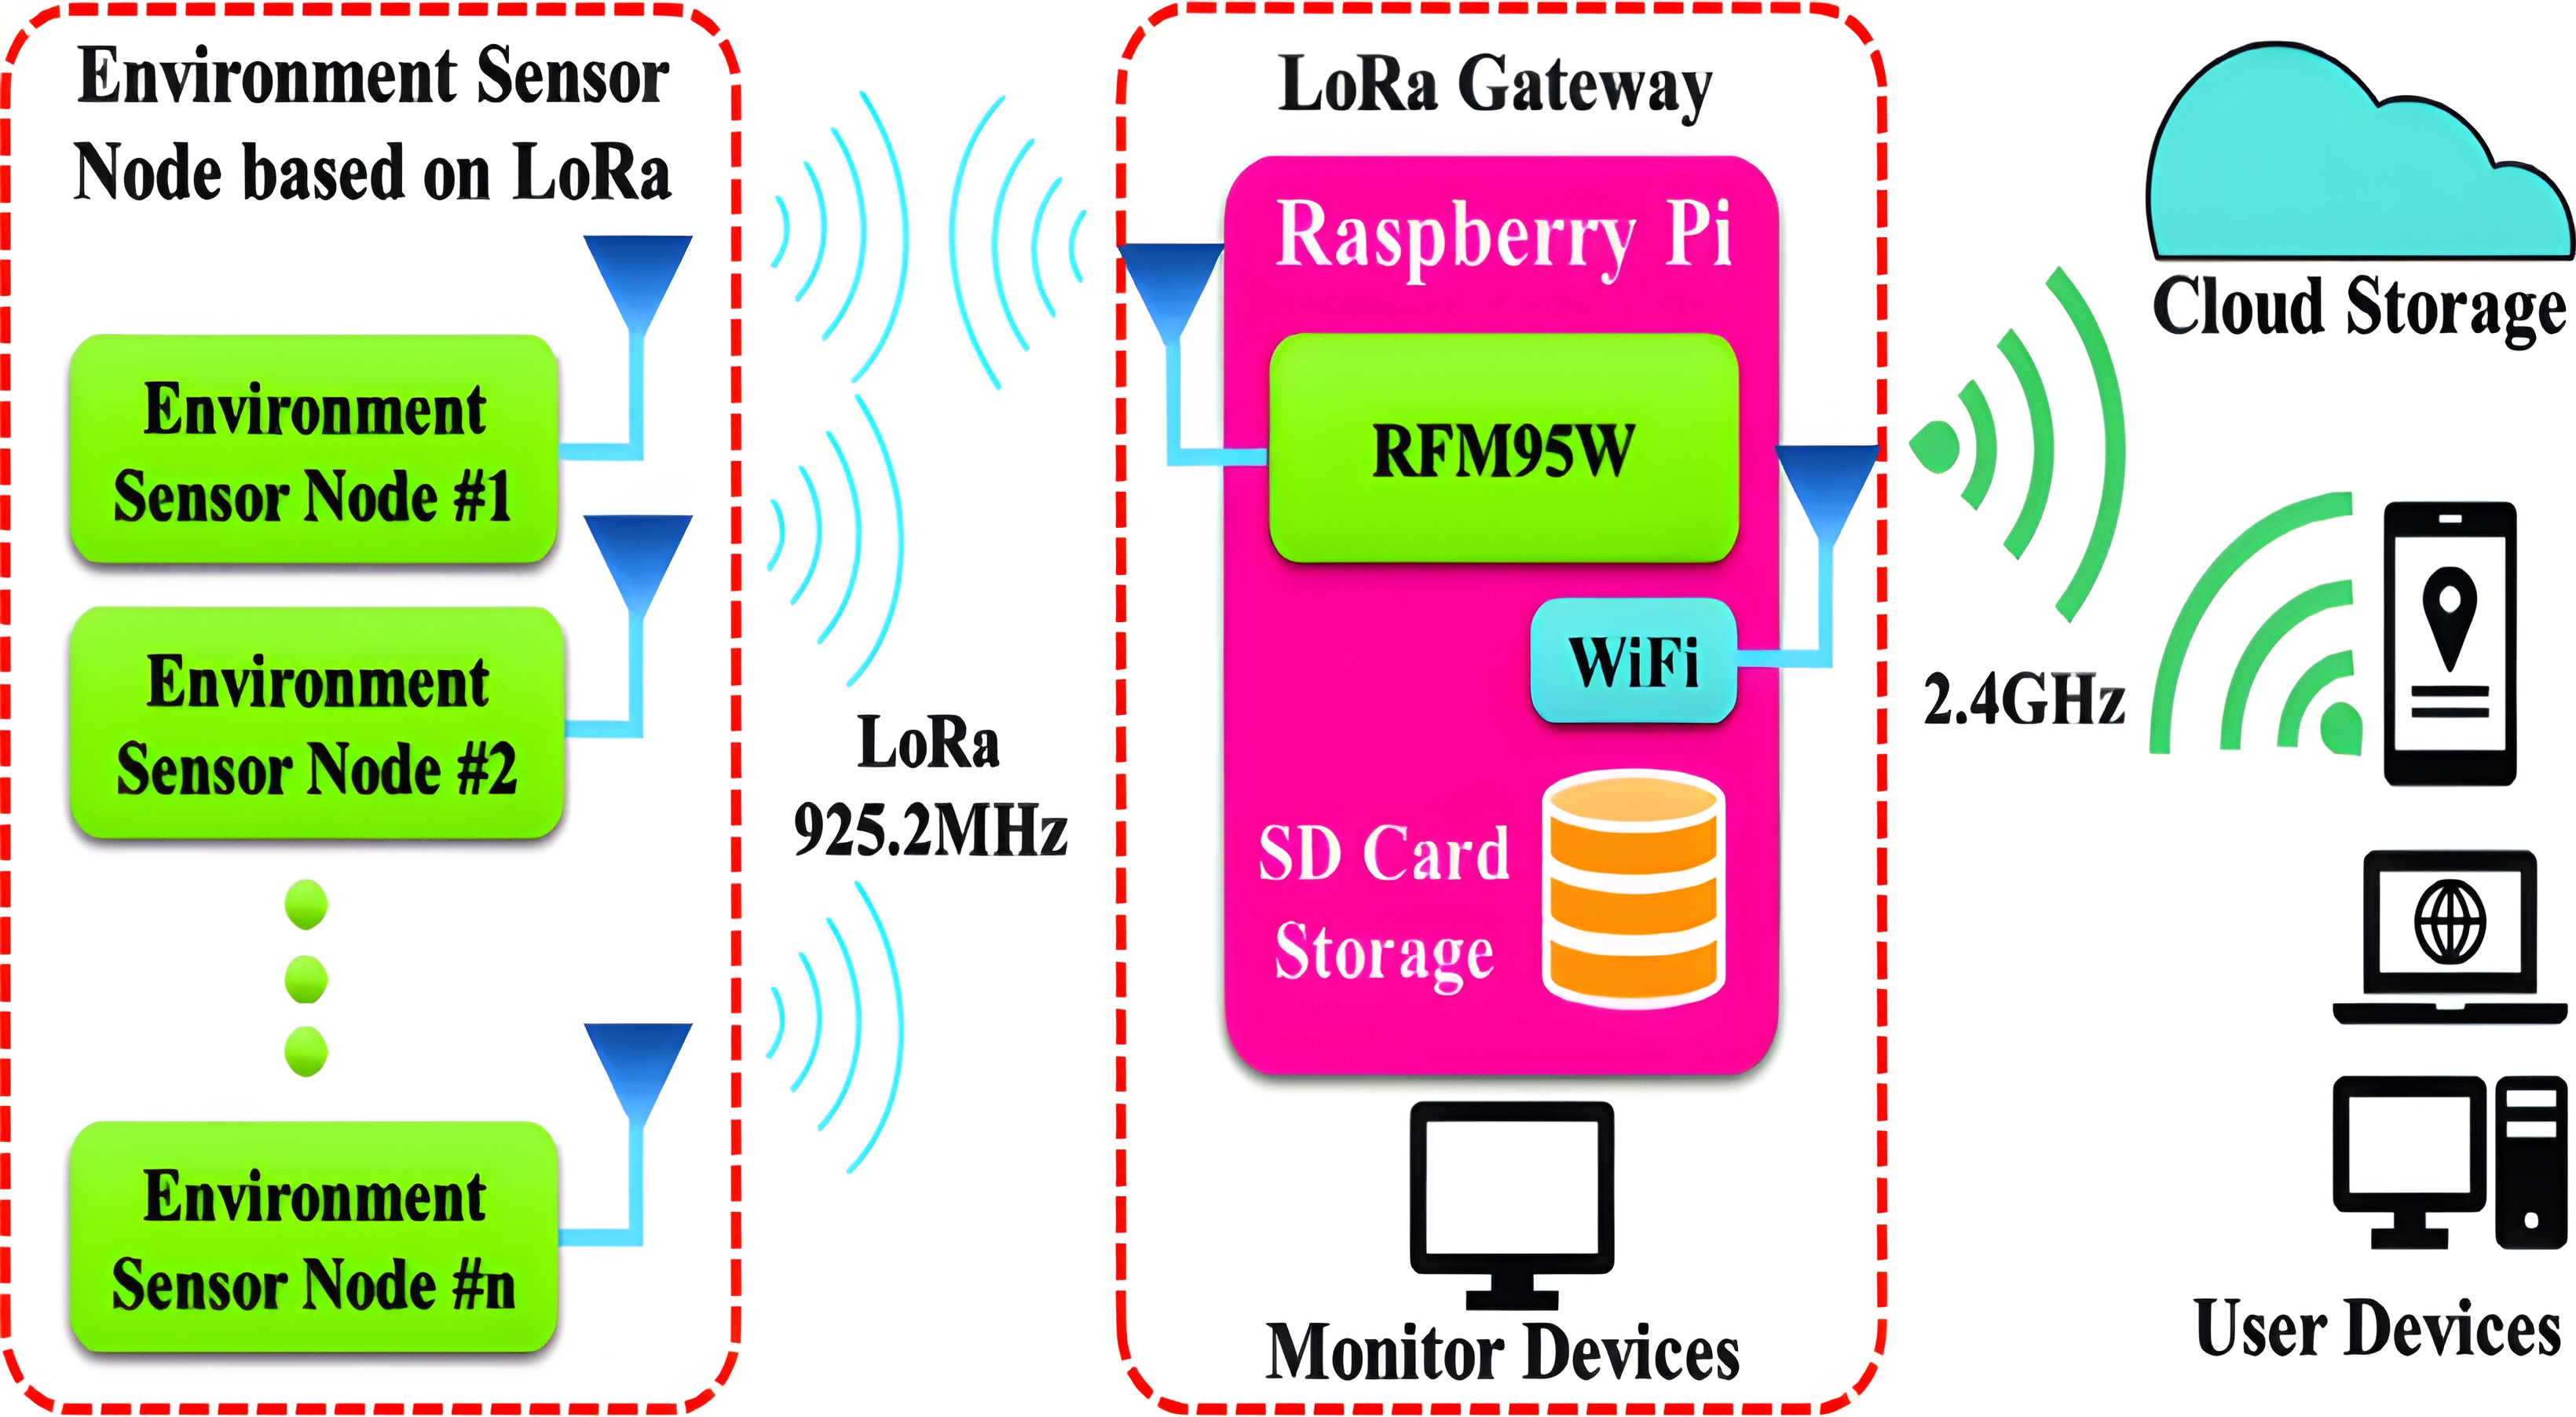
\includegraphics[scale=0.1]{Sections/Introduction/LoRaWAN-IOT-Example.jpg}
\end{figure}


\subsection{LoRa and LoRaWAN}
Low Power Wide Area Network (LPWAN) is a communication technology that offers wide coverage, similar to satellite networks, while maintaining lower data rates akin to ZigBee. The technology is distinguished by its ultra-low power consumption and cost-effective deployment and maintenance  \cite{IOTandLORAWAN-SmartFarm}.\\\\
LoRa and LoRaWAN, forms of LPWAN technology, were developed to overcome the scalabilty issues associated with traditional WSN configurations that relied on short-range communication protocols such as Zigbee and Bluetooth \cite{WSN-WaterQual}. These configurations often used a mesh network layout, which introduced challenges in network management and power consumption with increasing network size \cite{IOTandLORAWAN-SmartFarm}.\\\\
LoRaWAN's unique `star of stars' configuration addresses these challenges by enabling scalable network expansion with reduced complexity. LoRa itself is a Chirp Spread Spectrum (CSS) modulation technique developed by Cycleo, offering a Medium Access Control (MAC) protocol and operating on license-free, region-dependent Industrial, Scientific and Medical (ISM) frequency bands \cite{IOTandLORAWAN-SmartFarm}.

\begin{comment}
\begin{figure}[h]
	\centering 
	\caption{Comparison of main IoT enabling communication technologies in terms of range, data rate, energy consumption, and costs. \cite{IOTandLORAWAN-SmartFarm}}
	\label{IOTandLORAWAN-SmartFarm-Figure1}
	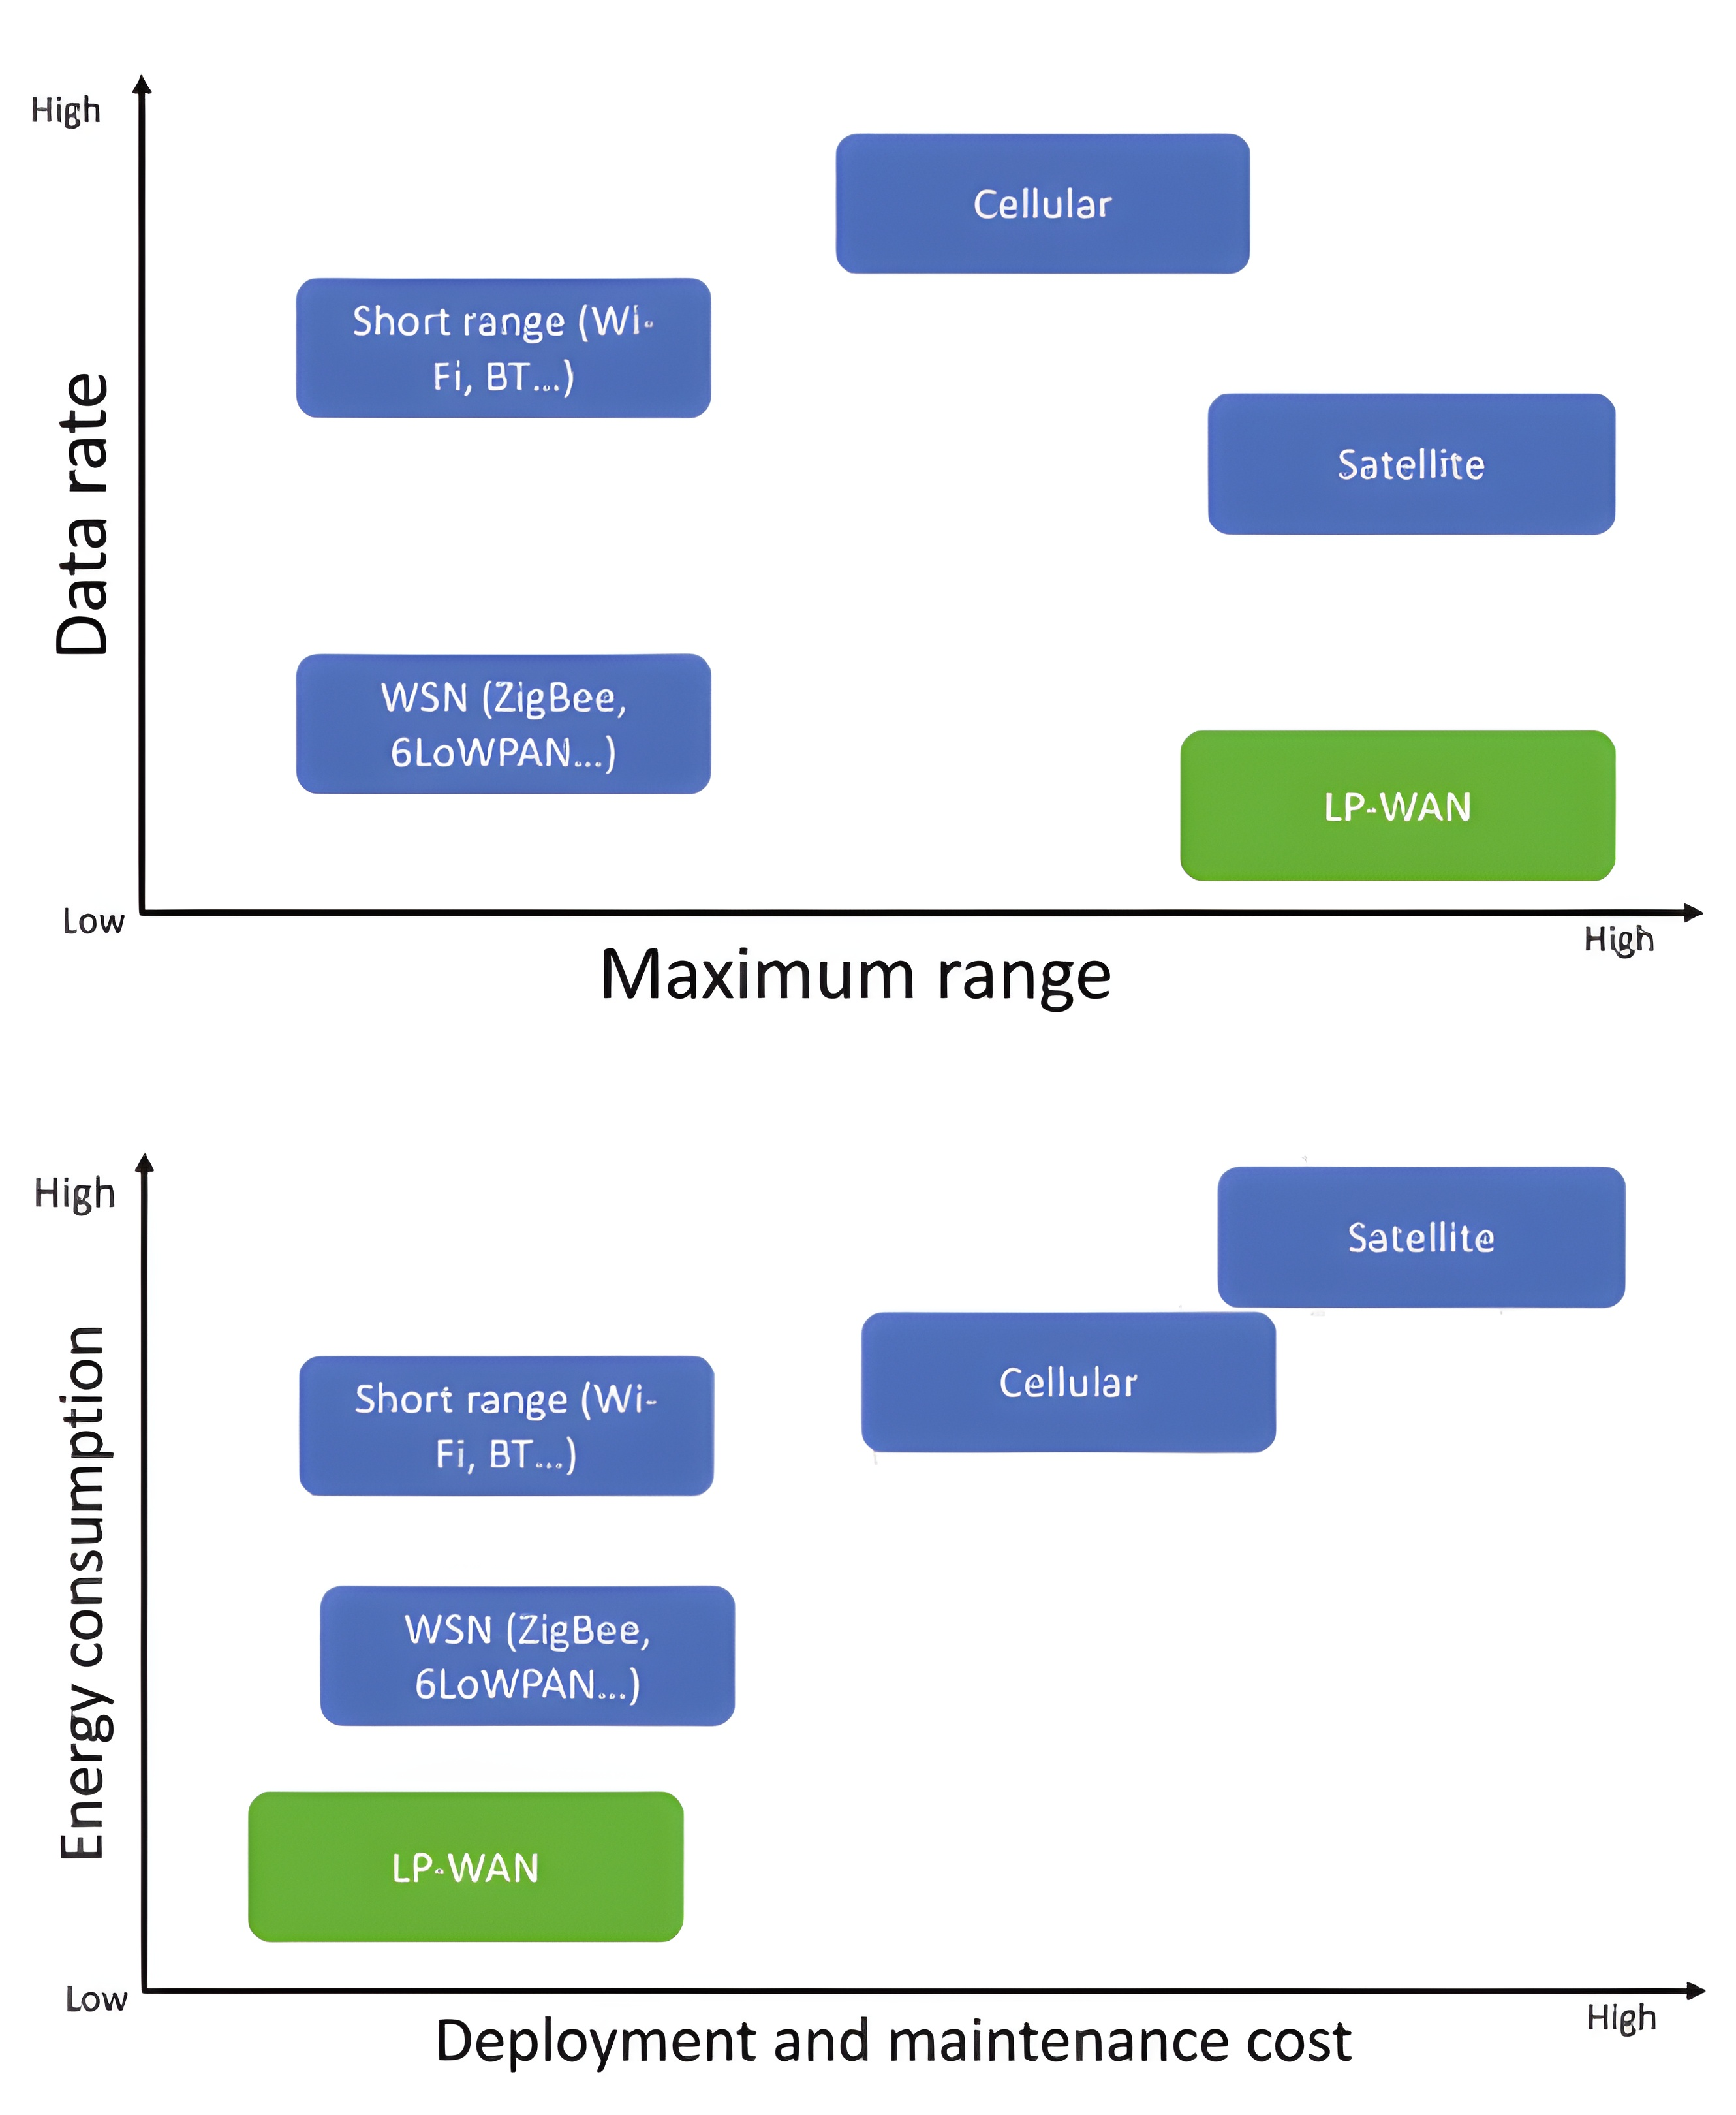
\includegraphics[scale=0.1]{Sections/Introduction/LP-WAN-Range.jpg}
\end{figure}
\end{comment}




\section{Aims and Objectives}
The aim of this IAP project is to develop an IOT system capable of collecting data relevant to further research regarding the health of the Griffith footbridge. The primary data acquisition units will come in the form of three sensor nodes placed across the footbridge that collect and process vibration data in three dimensions. The aim is to packetize this data and receive payloads at a gateway via the LoRaWAN transmission protocol. Finally, the data needs to be uploaded to the TNN Cloud for data processing and analysis. Figure \ref{fig:HL-HW-Diagram} exhibits the high level hardware diagram for the intended IoT system implementation. 


\begin{figure}[h!]
\center
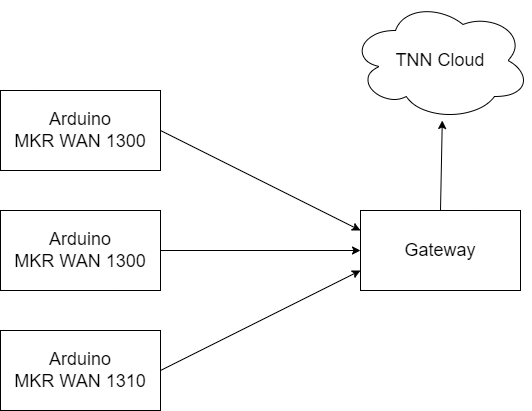
\includegraphics[scale=0.5]{Images/HW-Diagram.png}
\caption{High Level Hardware Diagram}
\label{fig:HL-HW-Diagram}
\end{figure}

The aims of this project will be satisfied once the following objectives are met.
\begin{enumerate}
\item Verify that the components selected for the IoT system are compatible and capable of transmitting and receiving data. 
\item Integrate an accelerometer into the system and write software that discretizes analog input data using the Fast Fourier Transform. 
\item Transmit the digital data from three different sensor nodes to the gateway. The gateway must be able to receive packets, identify the respective sensor node and upload the vibration payloads to the TNN cloud. 
\item Implement a solar system to constantly power the sensor nodes.
\item Design and implement a PCB carrier board for the sensor nodes.
\item Design and implement a 3D-printed enclosure to house the components of the sensor nodes. Figure \ref{fig:HL-HW-Diagram-Detailed} exhibits the detailed, high level, hardware system diagram and figure \ref{fig:HL-SW-Diagram} contains the high level, software diagram for the transmitter and receiver systems. 
\end{enumerate}

\begin{figure}[h!]
\center
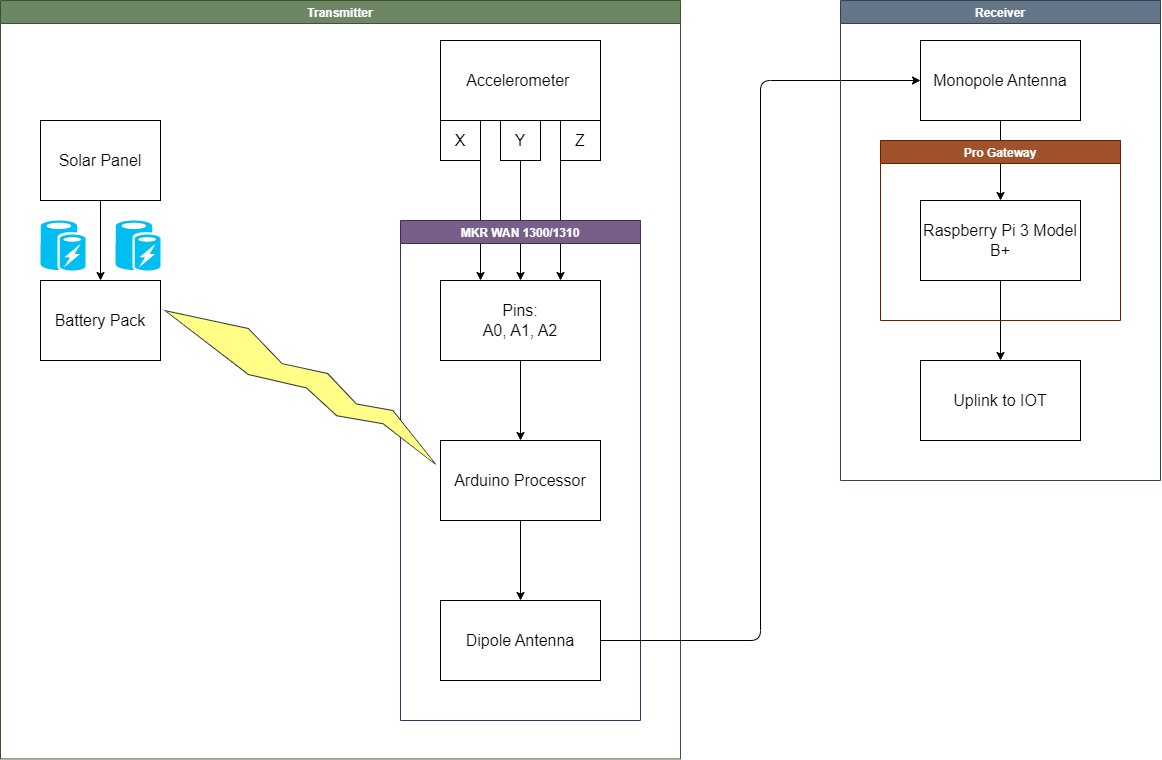
\includegraphics[scale=0.38]{Images/HW-Diagram-Detailed.png}
\caption{Detailed High Level Hardware Diagram}
\label{fig:HL-HW-Diagram-Detailed}
\end{figure}
\clearpage
\begin{figure}[h!]
\center
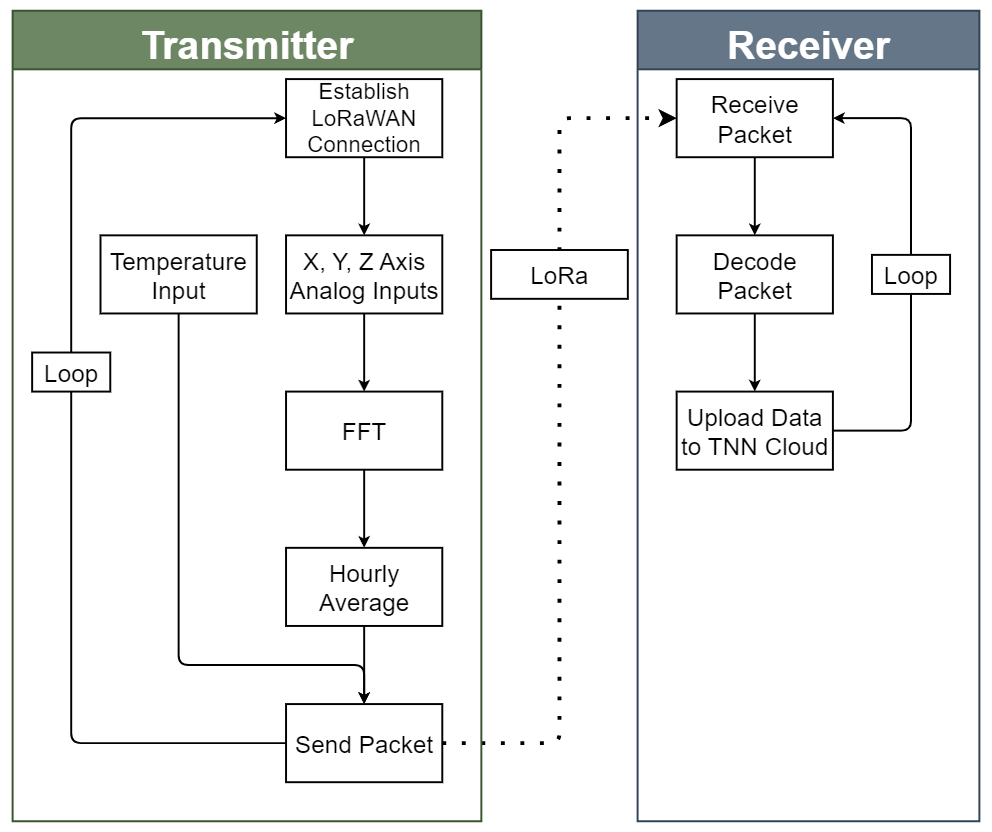
\includegraphics[scale=0.38]{Images/SW-Diagram.png}
\caption{High Level Software Diagram}
\label{fig:HL-SW-Diagram}
\end{figure}










\section{Expected Project Outcomes}
This project involves multiple outcomes that are confined within the scope of the project. The first outcome to meet is a proof of concept that satisfies the high level hardware and software diagrams. This will initially be completed with one sensor node and will achieve the objective of creating a functional IoT system in a closed loop environment. The next outcome to meet is introducing three sensor nodes into the system and writing the software to distinguish between each node's packets. To complete the closed loop testing the nodes will be placed on a test beam set up in the mechanical engineering labs that simulates vibration. Once the closed loop testing has been completed, the permanent implementation of the device will commence. This involves a solar-battery system sufficient of powering the low-powered devices at all times. Theoretical calculations and quantitative testing will be conducted to determine the power drain characteristics of these sensor nodes. Finally, an enclosure will be modeled and printed to house the electronics and power systems and will be used to mount the devices to the bridge. These enclosures also serve the purpose of weather-proofing the sensor nodes. The final outcome is to have a functional IoT system over the length of the Griffith footbridge that is capable of transmitting packets 24/7 to a gateway that will be placed up to 600m away. 

\input{Sections/Methodology-And-Schedule}
\clearpage
\section{Risk Assessment}
\subsection{Risk Assessment Risk Matrix}

\begin{longtable}[h!]{ | p{2.25cm} | p{2.25cm} | p{2.25cm} | p{2.25cm} | p{2.25cm} | p{2.25cm} | }\hline
& \multicolumn{5}{|c|}{\textbf{Consequences}}\\\hline
\textbf{Likelihood} & \textbf{Catastrophic (Cat)} & \textbf{Major (Maj)} & \textbf{Moderate (Mod)} & \textbf{Minor (Min)} & \textbf{Insignificant (Ins)} \\\hline
\textbf{Almost Certain (AC)} & \cellcolor{red}\textbf{Very High (VH)} & \cellcolor{red}\textbf{Very High (VH)} & \cellcolor{orange}\textbf{High (H)} & \cellcolor{yellow}\textbf{Medium (M)} & \cellcolor{green}\textbf{Very Low (VL)} \\\hline
\textbf{Likely (L)} & \cellcolor{red}\textbf{Very High (VH)} & \cellcolor{orange}\textbf{High (H)} & \cellcolor{yellow}\textbf{Medium (M)} & \cellcolor{lime}\textbf{Low (L)} & \cellcolor{green}\textbf{Very Low (VL)} \\\hline
\textbf{Possible (P)} & \cellcolor{orange}\textbf{High (H)} & \cellcolor{orange}\textbf{High (H)} & \cellcolor{yellow}\textbf{Medium (M)} & \cellcolor{lime}\textbf{Low (L)} & \cellcolor{green}\textbf{Very Low (VL)} \\\hline
\textbf{Unlikely (U)} & \cellcolor{yellow}\textbf{Medium (M)} & \cellcolor{yellow}\textbf{Medium (M)} & \cellcolor{lime}\textbf{Low (L)} & \cellcolor{green}\textbf{Very Low (VL)} & \cellcolor{green}\textbf{Very Low (VL)} \\\hline 
\textbf{Rare (R)} & \cellcolor{lime}\textbf{Low (L)} & \cellcolor{lime}\textbf{Low (L)} & \cellcolor{lime}\textbf{Low (L)} & \cellcolor{green}\textbf{Very Low (VL)} & \cellcolor{green}\textbf{Very Low (VL)} \\\hline
\caption{Risk Assessment Matrix}
\label{tab:RiskMatrix}
\end{longtable}

\begin{longtable}{ | P{3cm } | P{7cm} | }
\hline
\textbf{Risk Level}& \textbf{What should I do?} \\
\hline
\cellcolor{red}\textbf{Extreme}& Eliminate from activities \\
\hline
\cellcolor{orange}\textbf{High}& Eliminate from activities \\ 
\hline
\cellcolor{yellow}\textbf{Medium}& Specific monitoring or procedures required, management responsibility must be specified \\
\hline
\cellcolor{green}\textbf{Low}& Manage through routine procedures. Unlikely to need specific application of resources \\
\hline
\caption{Risk Level Management}
\label{tab:RiskManagement}
\end{longtable}

\clearpage
\subsection{Identified Risks} 

\begin{comment}
In table \ref{tab:RiskID}, (C) are consequences, (L) is likelihood and (LvL) is the level of risk.

\begin{longtable}{ | P{3.75cm} | P{3.5cm} | P{0.7cm} |  P{0.5cm} |  P{1cm} | P{3.75cm} | }
\hline
\textbf{What could cause harm?}& \textbf{What could go wrong?}& \textbf{C}& \textbf{L}& \textbf{LvL}& \textbf{What controls are required?} \\
\hline
Actively handling sensitive electronics& Risk of destroying components with ESD& \cellcolor{green}Ins& \cellcolor{green}R& \cellcolor{green}VL& Wear ESD wristband when handling sensitive electronics. \\
\hline
Soldering electronic connections& Burns and inhalation of solder fumes& \cellcolor{green}I& \cellcolor{green}R& \cellcolor{green}VL& Safety glasses and gloves. Extractor fans / ventilation. \\
\hline
Placing equipment on a tall footbridge over a busy highway& Dropping equipment onto the traffic below and causing an accident& \cellcolor{green}M& \cellcolor{green}U& \cellcolor{green}VL& Bridge has protective railing. Design a lightweight system and gain supervisor approval before field implementation. \\
\hline
Vibrating beam experiment& Crushing or physical injury& \cellcolor{green}I& \cellcolor{green}R& \cellcolor{green}VL& Wear enclosed footwear. Ensure surroundings are clear. Keep distance whilst experiment is running. \\
\hline
\caption{Identified Risks}
\label{tab:RiskID} 
\end{longtable}
\end{comment}

\begin{figure}[h!]
\centering
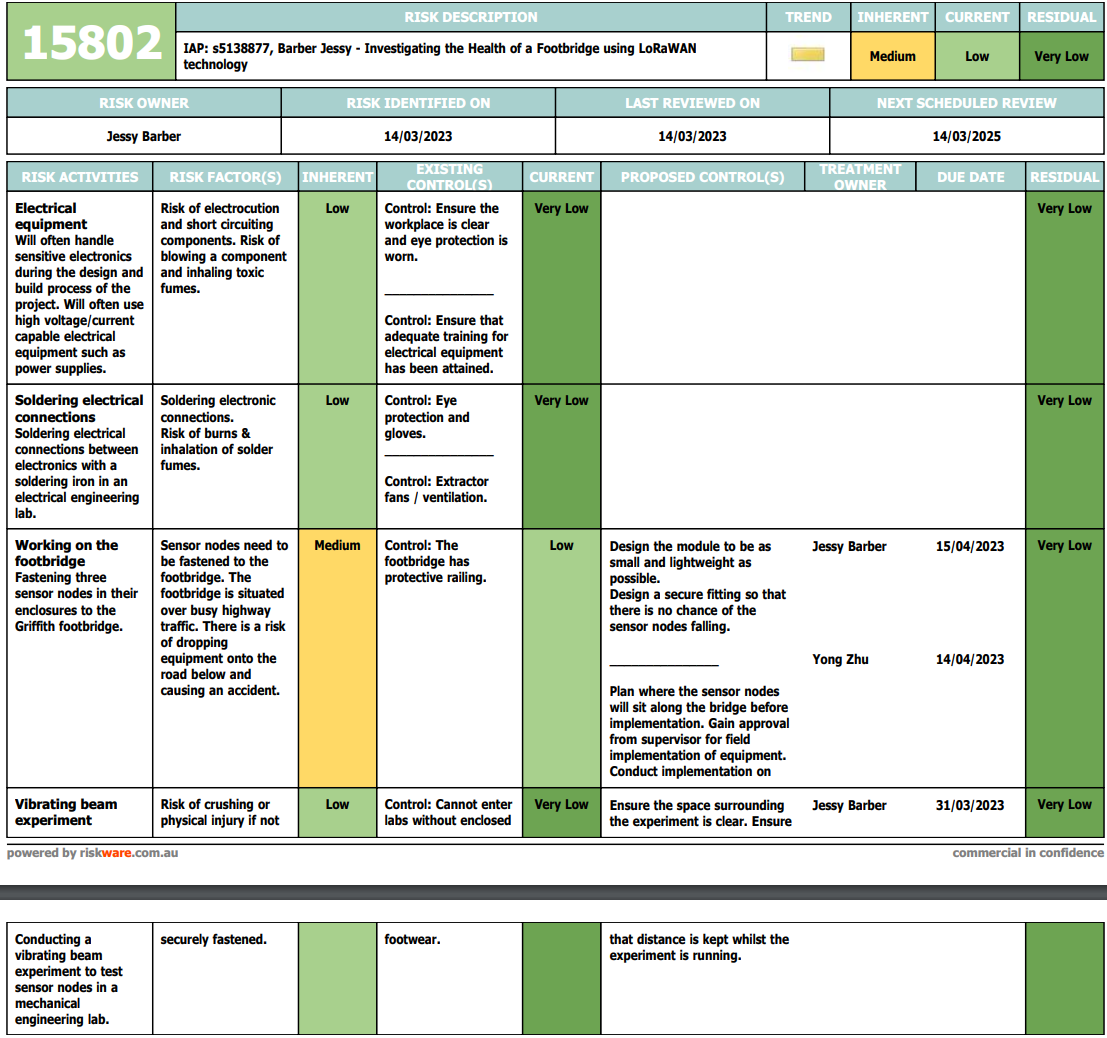
\includegraphics[scale=0.6,angle=90,origin=c]{Images/Risks.png}
\caption{GSAFE Risk Assessment}
\label{fig:GSAFE}
\end{figure}




\section{Ethics Issues Related to the Project}


\bibliographystyle{IEEEtran}
\bibliography{References}

\end{document}